\section{Referencial teórico}

Esta seção explora os fundamentos que sustentam o desenvolvimento de um sistema médico distribuído de alta disponibilidade.
Para contextualizar a proposta, serão abordados conceitos fundamentais sobre imagens microscópicas, o papel das redes neurais convolucionais na análise visual, a técnica de segmentação de imagens e uma revisão de trabalhos relacionados na área de sistemas CAD para análise de imagens médicas.

O avanço na criação dos algoritmos usados nos sistemas CAD tem sido enriquecido por contribuições de múltiplos campos do conhecimento, incluindo a filosofia, matemática, economia, neurociência, psicologia, engenharia da computação, linguística, teoria do controle e cibernética, destacando o caráter interdisciplinar que caracteriza o campo da IA. Segundo \cite{10.5555/1671238}, a Inteligência Artificial  é um campo da computação que se dedica ao desenvolvimento de agentes inteligentes, máquinas com aparente capacidade de raciocínio semelhante ao humano. Logo, a inteligência artificial, também envolve o treinamento desses agentes inteligentes. A subárea da IA que é responsável por explorar os algoritmos para o desenvolvimento desses agentes se chama aprendizado de máquina. 

Nesse campo de estudo, existem três abordagens distintas de aprendizados, o aprendizado supervisionado, onde o agente reconhece padrões mesmo sem ter recebido valores de saída explícitos; aprendizado por reforço, no qual o sistema aprende a partir de diversos estímulos, que funcionam como sinais para as decisões do agente, sejam estes negativos em caso de uma predição incorreta, ou positivos no caso de uma boa decisão; e por último, o aprendizado supervisionado, esse tipo de aprendizado é muito popular no treinamento das redes neurais convolucionais; nessa técnica de aprendizado, o agente recebe os dados de entrada e saída, e ao decorrer das iterações a IA aprende a função que mapeia a entrada com a saída \cite{haykin2009neural}.

A aplicação de algoritmos de aprendizado de máquina terá um impacto significativo neste estudo, permitindo que a rede reconheça os padrões e segmente a região das células. Será enfatizado a aplicação de uma categoria específica de algoritmos denominado aprendizado profundo (Deep learning (DL)), esse campo de estudo compreende uma vasta família de técnicas de aprendizado de máquina, nas quais as hipóteses são representadas por circuitos algébricos de elevada complexidade, com parâmetros de conexão ajustáveis. O termo ‘profundo’ refere-se ao fato de que esses sistemas geralmente estão organizados em camadas \cite{10.5555/1671238}. Esses circuitos conectados são conhecidos como redes neurais artificiais e são compostos por interconexões de um modelo matemático chamado \textit{perceptron}, que por sua vez tem seu funcionamento inspirado pelo neurônio humano.

\begin{figure}[h]
\centering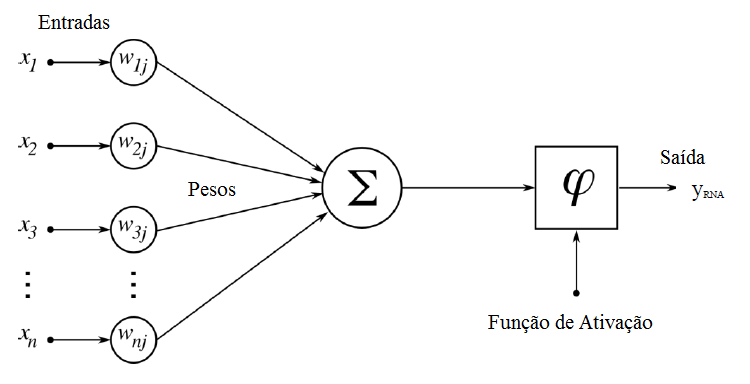
\includegraphics[scale=0.4]{images/Figura-1-neuronio-artificial.png}
\caption{Exemplo do modelo perceptron \cite{imagemperceptron}.}
\label{fig: perceptron}
\end{figure}


O perceptron, demonstrado na Figura \ref{fig: perceptron}, foi inicialmente proposto por Frank Rosenblatt em 1957 como um classificador linear inspirado em neurônios biológicos, é uma unidade de processamento que recebe entradas \(x\) ponderadas pelos pesos \(w\), essa operação inicial pode ser representada como

\begin{equation}
  \(z = \sum_{i=1}^{n} w_i x_i\) \;.
  \label{eq:percetron}
\end{equation}

Posteriormente, a rede processa essas entradas por meio de uma função de ativação, a função de ativação tem a responsabilidade de amplificar o aprendizado do sistema, visto que por meio dessa função o neurônio será ativado ou não. A função de ativação aplica uma transformação não linear a saída da primeira operação \(z\), que é representada no final por \(\sigma = f(z + b)\), sendo \(b\) um termo de viés. Durante o treinamento, o perceptron ajusta seus pesos \(w_i\) com base no erro entre a previsão e o valor esperado. A regra de aprendizado é dada pela fórmula

\begin{equation}
  w_i = w_i + \Delta w_i
  \label{eq:Referencial}
\end{equation}

\noindent em que \(\Delta w_i = \eta(y_{esperado} - y_{previsto})\), sendo \(\eta\) o valor da taxa de aprendizado, que controla a magnitude da atualização dos pesos. Esse ajuste permite que ao decorrer das iterações o perceptron modifique suas conexões para melhorar seu desempenho em tarefas de calssificação \cite{haykin2009neural}. De maneira isolada, o perceptron possui a limitação de resolver apenas problemas linearmente separáveis, já a combinação de múltiplos perceptrons em camadas, conhecida como \textit{Multi Layer Perceptron} (MLP),  permite que esse modelo aproxime funções não lineares complexas.

\begin{figure}[h]
\centering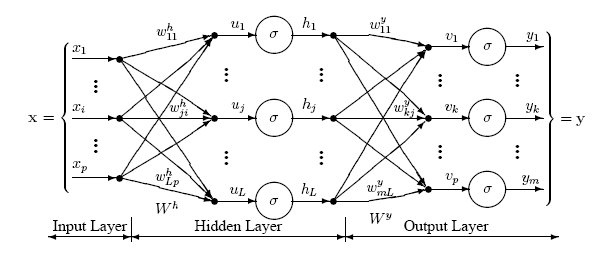
\includegraphics[scale=0.75]{images/mlp.jpg}
\caption{Exemplo do modelo \textit{multi layer perceptron} (DTREG, 2024).}
\label{fig: mlp}
\end{figure}


Para \citeonline{haykin2009neural}, o MLP é um modelo baseado em aprendizado supervisionado, onde o objetivo é minimizar o erro na camada de saída. O MLP representa uma extensão do perceptron, cada camada do MLP realiza uma transformação não linear dos dados, assim, permite a captura de interações complexas entre as camadas. Exemplificado na figura \ref{fig: mlp}, as redes MLP são divididas em três partes: A camada de entrada, que possui a responsabilidade de receber os dados iniciais; as camadas intermediárias ou camadas ocultas (\textit{hidden layers}), que processam essas informações; e a camada de saída, onde é gerado os valores de saída da rede. Para atingir o objetivo de minimizar o erro, o sistema utiliza um algoritmo de retropropagação (\textit{backpropagation}) que foi proposto por \citeonline{Rumelhart1986-zt}.Esse algoritmo tem por objetivo ajustar os pesos ao longo das camadas, propagando o erro da camada de saída até as camadas intermediárias. Esse algoritmo utiliza a regra da cadeia para calcular o gradiente do erro em relação a cada peso da rede, facilitando o ajuste dos pesos para minimizar o erro. Esse algoritmo tem sua operação é divida em duas fases: a passagem para frente (\textit{forward pass}) e a passagem para trás (\textit{backward pass}). Na etapa da passagem para frente, a rede recebe uma amostra de entrada e propaga os valores através das camadas para gerar uma predição, ao final da rede, uma saída é gerada e comparada ao valor esperado, gerando um erro que será minimizado na próxima etapa. 

Contudo, no contexto de análise de imagens, há uma arquitetura de redes neurais mais especializada para entradas de imagens, essa arquitetura é denominada de redes neurais convolucionais (\textit{Convolutional Neural Network} (CNN)). As redes convolucionais são uma classe especial de redes neurais, desenvolvidas especificamente para o processamento de dados estruturados em grades, como imagens. As CNN, inicialmente propostas por \citeonline{6795724}, por meio de uma pesquisa para o reconhecimento de dígitos manuscritos, se tornaram uma das principais abordagens em visão computacional. Essa arquitetura de sistema envolve a composição das redes MLP com técnicas de processamento digital de imagens, como a convolução. A convolução é um processo de filtragem espacial (plano que contém os pixels da imagem), que consiste em aplicar o somatório do produto entre duas funções, a imagem e uma máscara ao longo da região que estas se sobrepõem, sendo a imagem uma função bidimensional f(i,j), em que i e j são as coordenadas, e a amplitude de f em qualquer par de coordenadas se refere a intensidade de cor naquele ponto, já a máscara é uma matriz de tamanho variado \cite{gonzalez2008digital}. 

\begin{figure}[h]
    \centering
    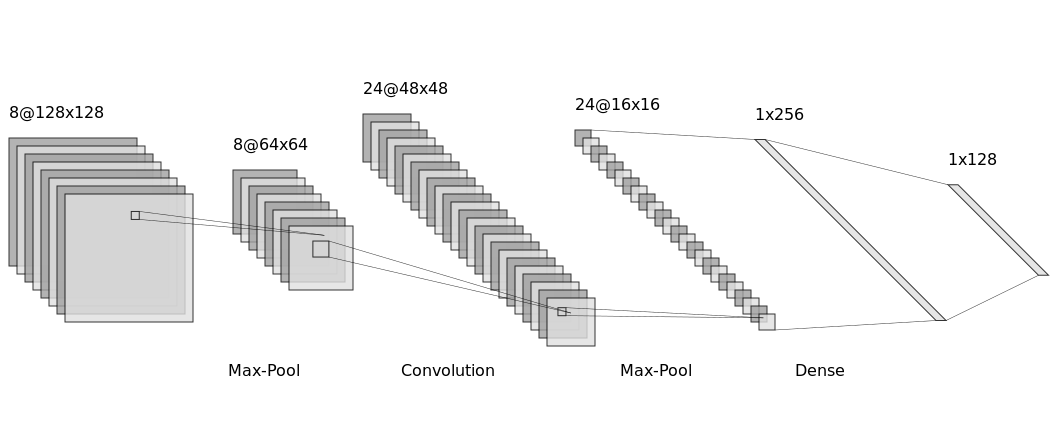
\includegraphics[scale=0.4]{images/redeconv.png}
    \caption{Exemplo rede neural convolucional (CORRÊA, 2024).}
    \label{fig: cnn}
\end{figure}

A figura \ref{fig: cnn} representa uma arquitetura típica de uma CNN, geralmente compostas por camadas convolucionais, de Pooling, totalmente conectadas e uma camada de saída. Cada uma dessas camadas realiza uma tarefa diferente, sendo as camadas convolucionais responsáveis pela atividade de extração de características, como bordas e texturas; a camada de Pooling é utilizada para reduzir a dimensionalidade dos dados; e por último, as camadas totalmente conectadas ou redes MLP que tem o mesmo funcionamento conforme apresentado anteriormente. 

A partir desse tipo de algoritmo, é possível se estender a tarefas mais avançadas que vão além da classificação de imagens, como por exemplo a segmentação de imagens. A tarefa de segmentação subdivide uma imagem em regiões ou objetos que a compõem. O nível de detalhe em que a subdivisão é realizada depende do problema a ser resolvido. O processo de segmentação deve parar quando os objetos ou as regiões de interesse de uma aplicação forem detectados \cite{gonzalez2008digital}. \citeonline{gonzalez2008digital} apontam que a segmentação de imagens é uma das tarefas mais difíceis no processamento de imagens, já que a precisão da segmentação determina o sucesso ou fracasso final dos procedimentos de análise computadorizada.

No contexto clínico, a utilização de dados visuais é indispensável para o diagnóstico da doença. A utilização desses sistemas é fundamental, visto que, diferente dos seres humanos, que são limitados à banda visual do espectro eletromagnético(EM), os aparelhos de processamento de imagem cobrem quase todo o espectro EM, variando de ondas gama a ondas de rádio. Esses sistemas podem trabalhar com imagens geradas por fontes que os humanos não estão acostumados a associar, como microscopia eletrônica, ultrassom e imagens geradas por computador \cite{gonzalez2008digital}.

Para o sistema proposto, o foco recai sobre a análise de dados obtidos através da microscopia, uma técnica fundamental para a visualização e o estudo detalhado de estruturas biológicas em nível celular. Na microscopia moderna existem algumas técnicas já bem estabelecidas, como a microscopia de fluorescência, em que é utilizada a luz ultravioleta para a geração dessas imagens - a tarefa básica do microscópio de fluorescência é utilizar uma luz de excitação para irradiar um espécime preparado e depois separar a luz fluorescente irradiante, muito mais fraca, da luz de excitação, mais intensa. A figura \ref{fig: fluomicro} apresenta um exemplo de microscopia de fluorescência. 

\begin{figure}[h]
  \centering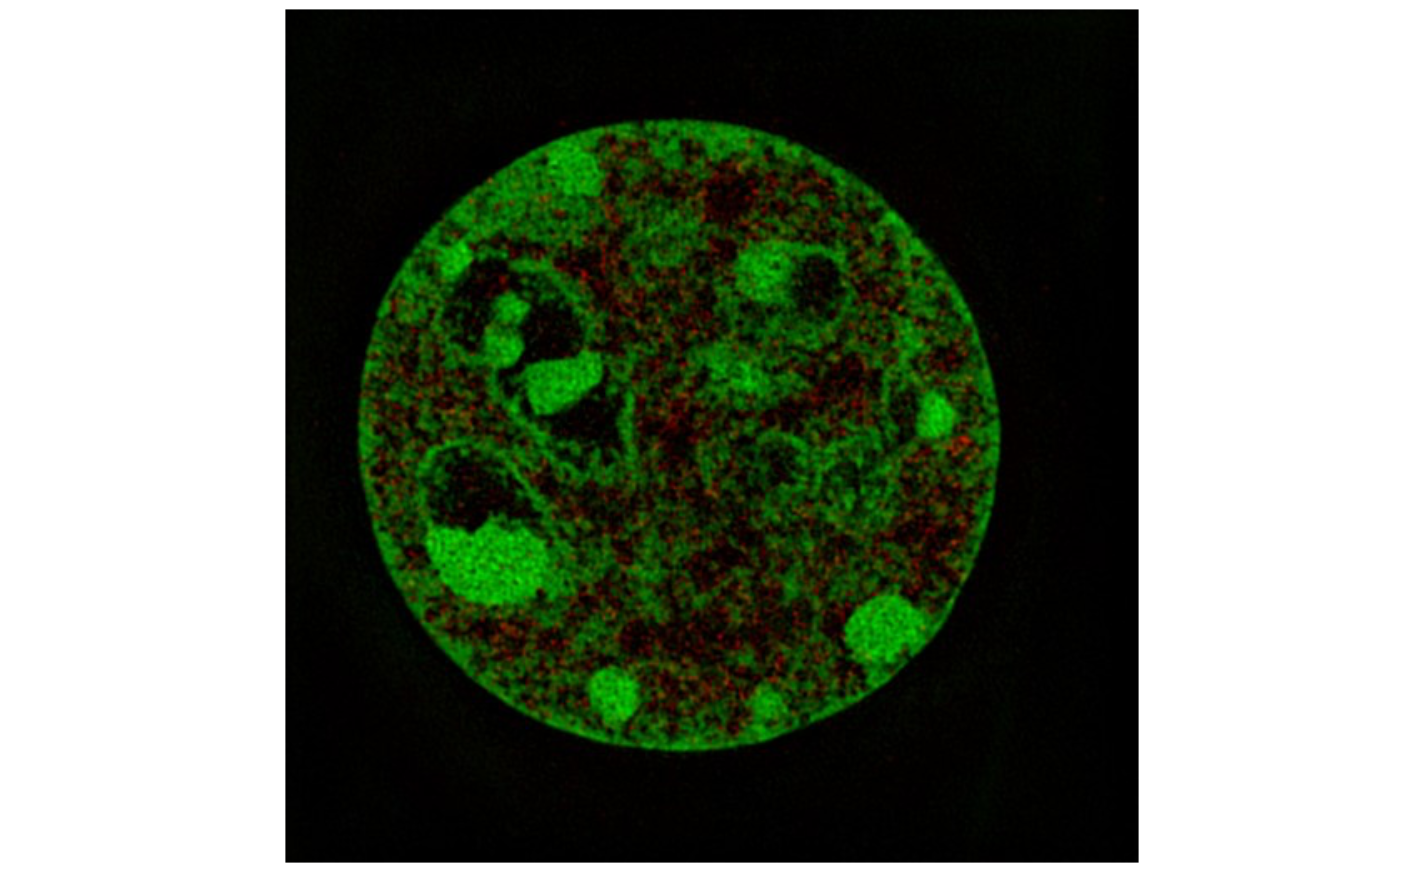
\includegraphics[scale=0.18]{images/fluo-micro.png} 
  \caption{Imagem de microscopia fluorescente \cite{fluo-micro}.}
\label{fig: fluomicro}
\end{figure}

Dessa forma, só a luz de emissão atinge o olho ou outro detector. As áreas fluorescentes resultantes brilham contra um fundo escuro com contraste suficiente para permitir a detecção. Quanto mais escuro for o fundo do material não fluorescente, mais eficiente é o instrumento \cite{gonzalez2008digital}.

Em contraste, a microscopia óptica, também definido por \citeonline{gonzalez2008digital}, utiliza a luz visível transmitida ou refletida através da amostra e um sistema de lentes para ampliar a imagem, sendo essencial para a análise morfológica de células sanguíneas e tecidos, demonstrado na figura \ref{fig: opticalmicro}.

% \begin{figure}[h]
%   \centering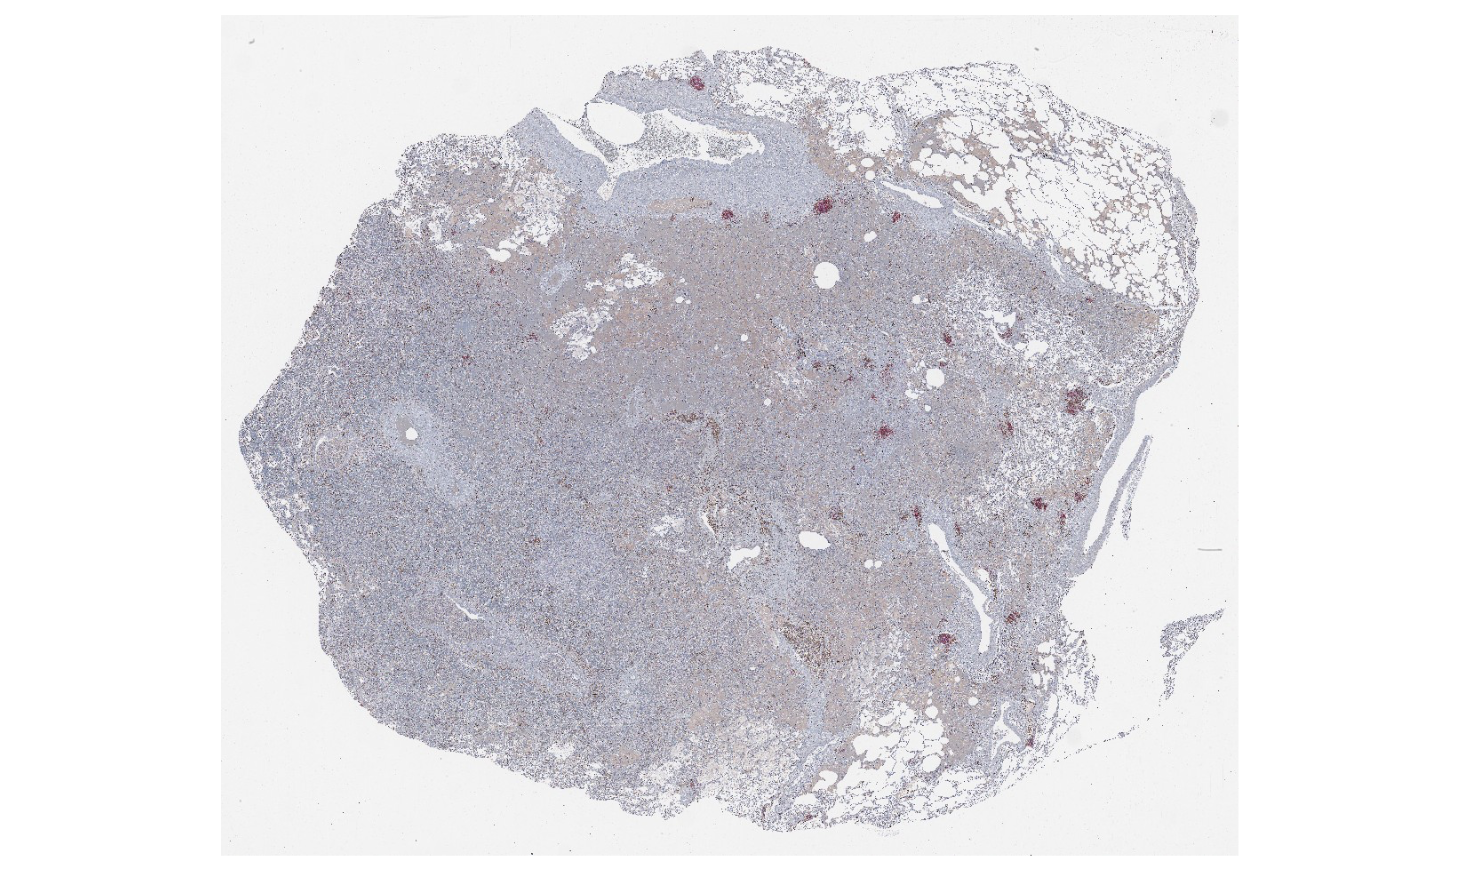
\includegraphics[scale=0.18]{images/lung06.png}
% \caption{Imagem de microscopia óptica \cite{Schaadt2020}.}
% \label{fig: opticalmicro}
% \end{figure}

\begin{figure}[h]
  \begin{subfigure}{0.5\textwidth}
    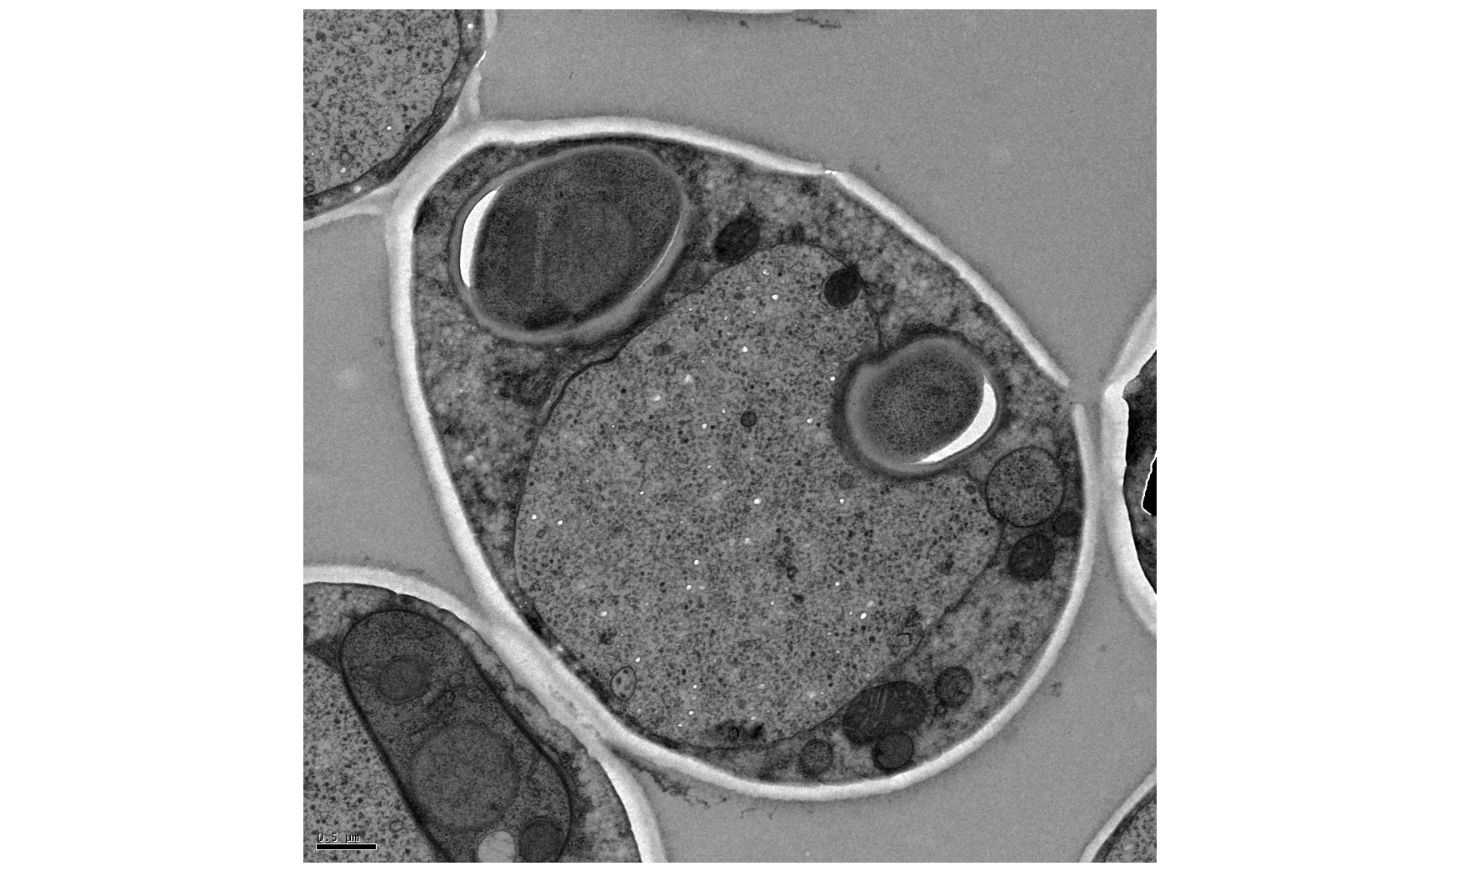
\includegraphics[scale=0.16]{images/electron_micro} 
    \caption{Imagem de microscopia eletronica \cite{eletron-micro}}
    \label{fig: electronmicro}
  \end{subfigure}
% \hfill
  \begin{subfigure}{0.5\textwidth}
    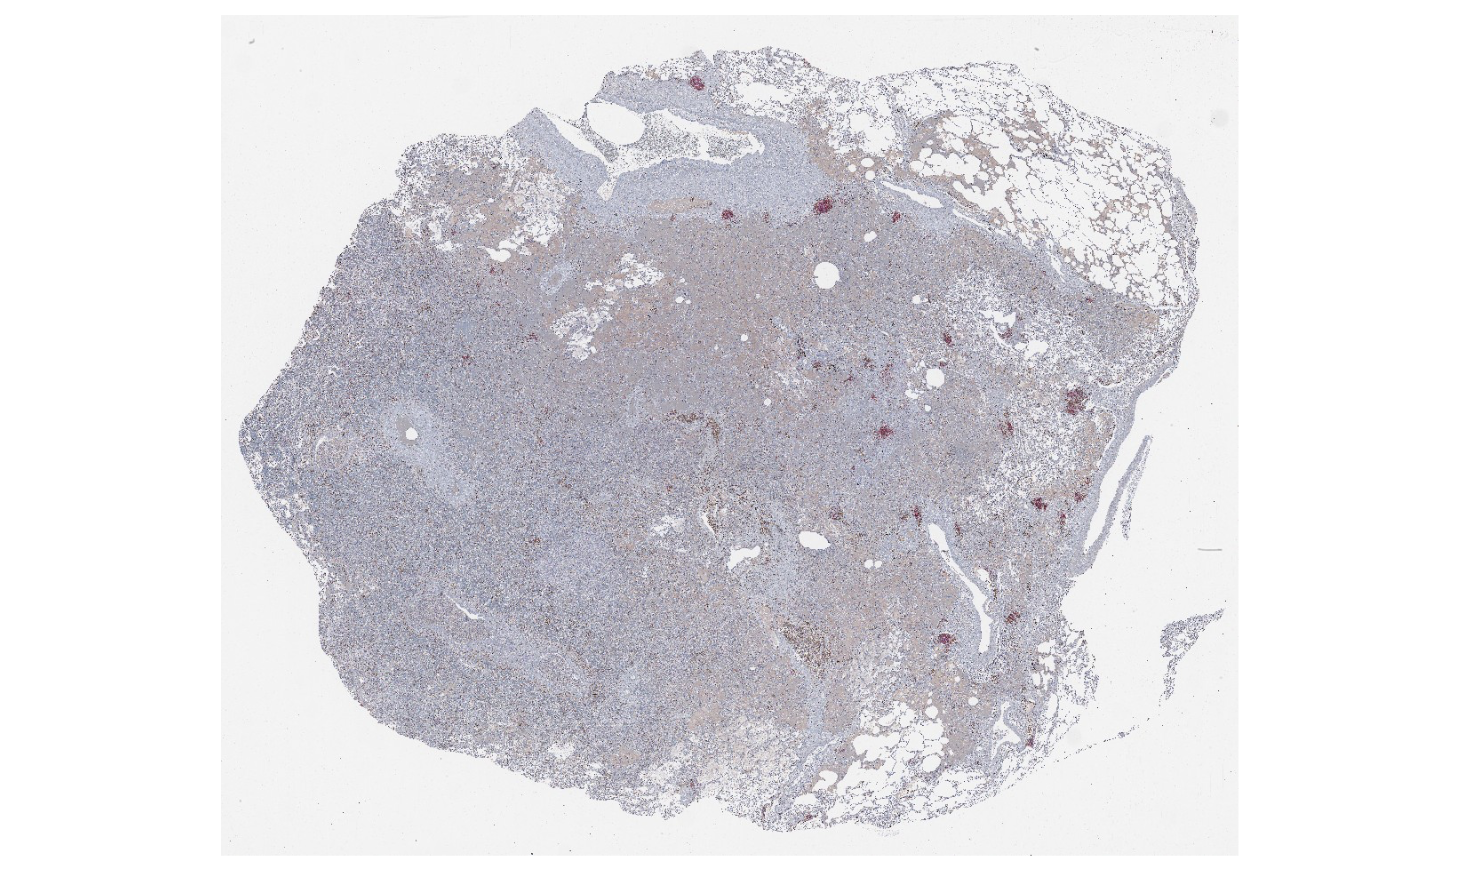
\includegraphics[scale=0.16]{images/lung06}
    \caption{ Imagem de microscopia óptica \cite{Schaadt2020}.}
    \label{fig: opticalmicro}
  \end{subfigure}
\caption{Exemplo de amostras de microscopia}
\label{fig: microimg}
\end{figure}


E por último os microscópios eletrônicos - figura \ref{fig: electronmicro} - que operam como seus correspondentes óticos, mas utilizam um feixe concentrado de elétrons em vez de luz para criar a imagem de uma amostra, permitindo resoluções muito maiores devido ao menor comprimento de onda dos elétrons. Essas imagens microscópicas são essenciais para diversas análises científicas e médicas, e é justamente a partir delas que sistemas avançados, como os sistemas de detecção auxiliada por computador, podem ser treinados para identificar padrões e auxiliar no diagnóstico médico.

% \begin{figure}[h]
%   \centering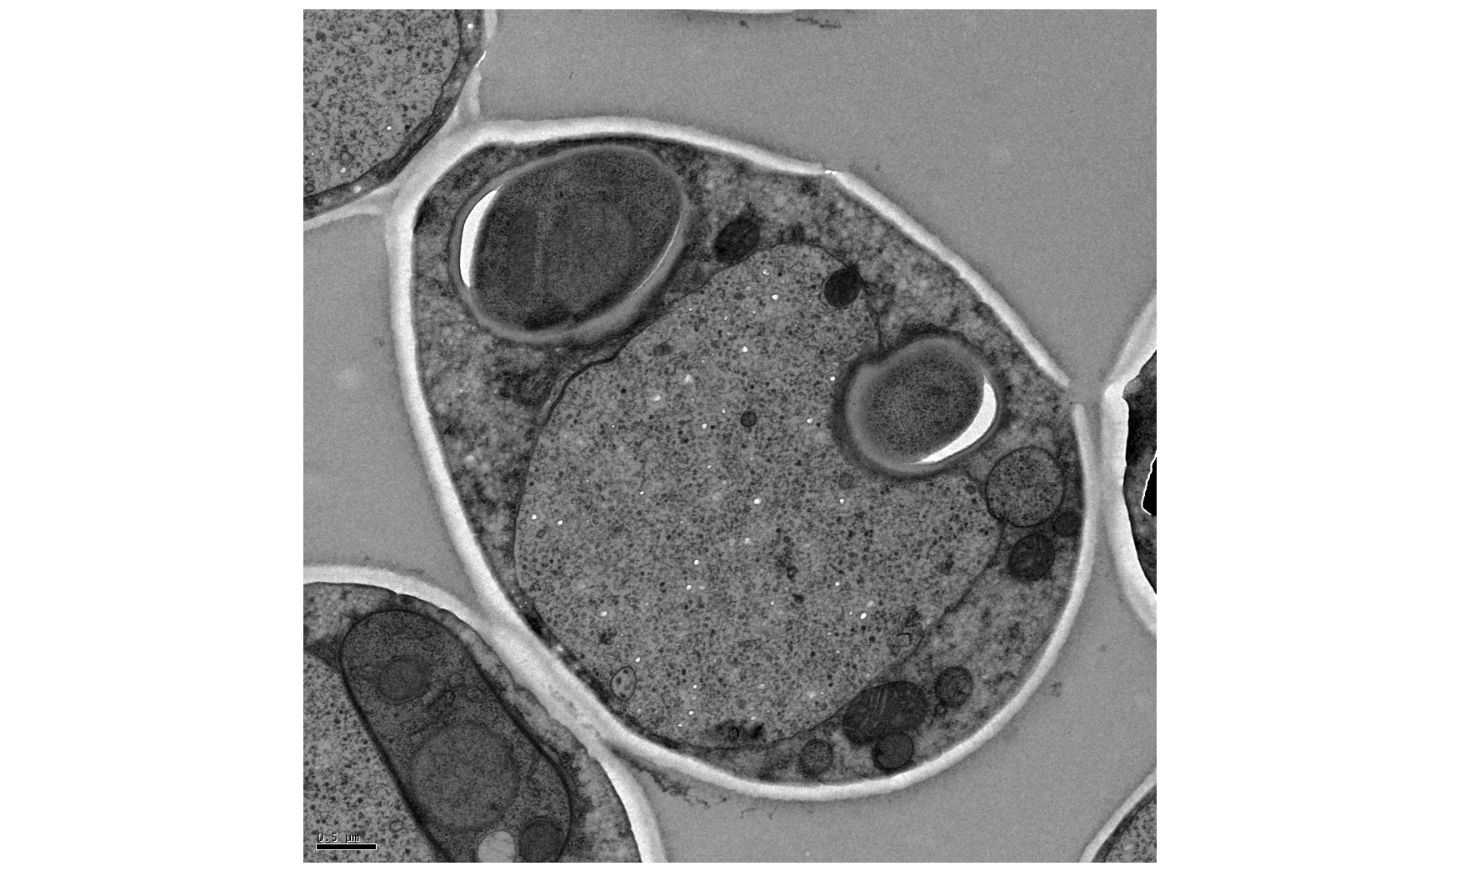
\includegraphics[scale=0.2]{images/electron_micro.png}
%
%   \centering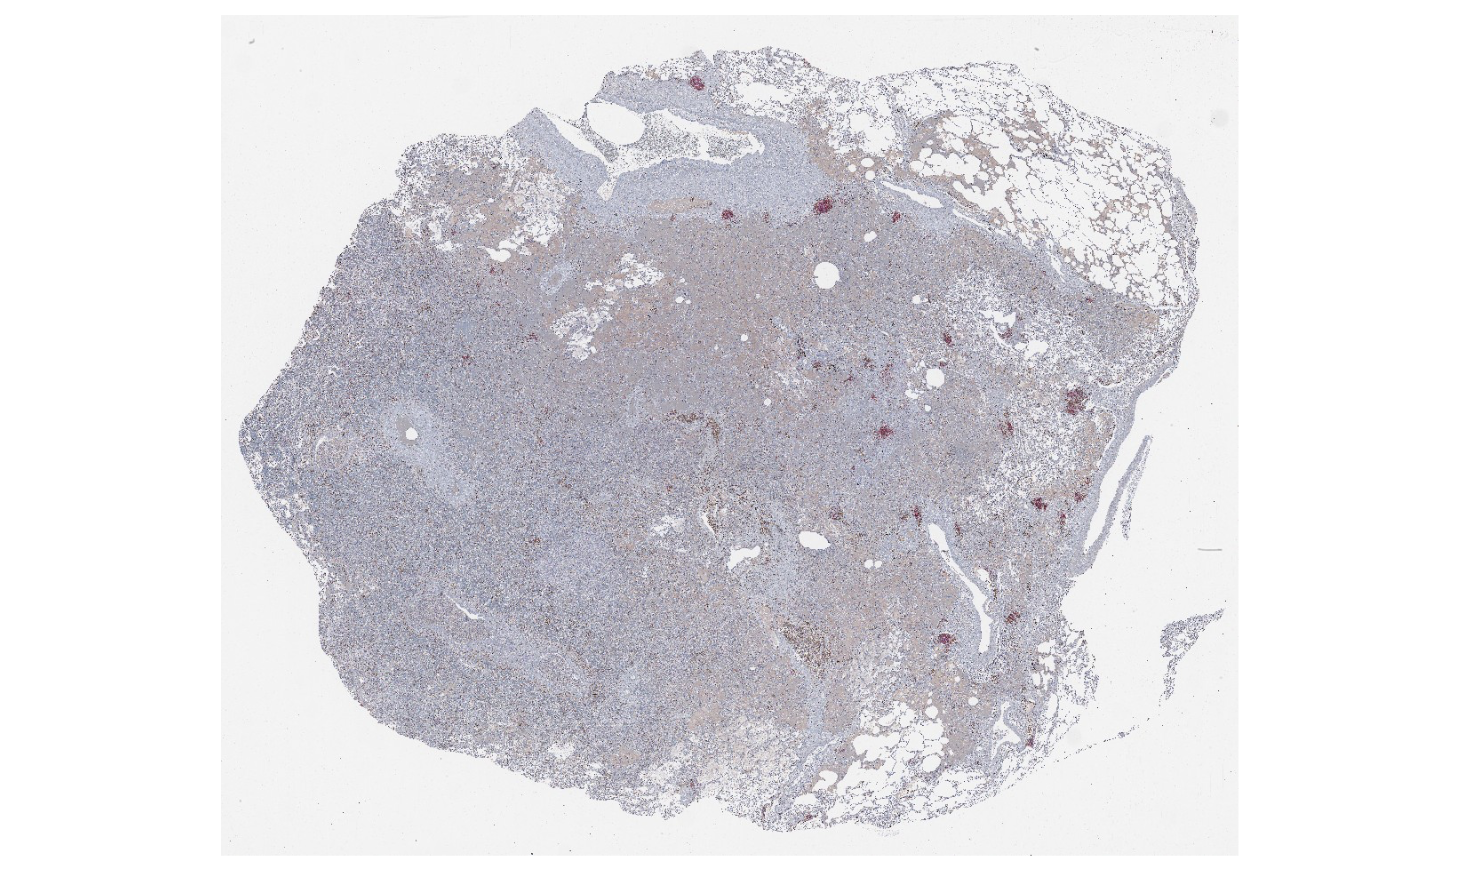
\includegraphics[scale=0.18]{images/lung06.png}
% \caption{Imagem de microscopia eletronica \cite{eletron-micro}.}
% \label{fig: electronmicro}
% \end{figure}


% Imagens microscopicas podem ser geradas de diferentes maneiras, entretanto no geral elas são formadas a partir do apoio de um dispositivo microscopico, que emite feixes de luz sob a materia sendo analisada, e todo esse processo é capturado por lentes com uma alta capacidade 

Os primeiros estudos sobre sistemas de detecção auxiliada por computador (CAD) e técnicas de análise quantitativa de imagens médicas por computador foram relatados na década de 1960. No entanto, foi na década de 80 que emergiu uma nova perspectiva, que assume que esses sistemas possam ser utilizados de maneira complementar aos profissionais da área da saúde e não para substituí-los. 

Portanto, o objetivo desses sistemas se torna ser uma segunda opnião para os médicos, para que estes façam a sua avaliação final. Alguns estudos ainda indicam que os sistemas CAD não devem necessáriamente apresentar uam precisão na classificação de doenças superior aos profissionais na área da saúde. No entanto, é fundamental observar que um maior desempenho desses sistemas resulta num valor final combinado mais otimizado, proporcionando maior eficiência entre a análise humana e computacional \cite{DOI2007198}. Atualmente, os sistemas CAD exploram diversas técnicas de inteligência artificial e visão computacional. Para auxiliar no desenvolvimento desta pesquisa, foram pesquisados artigos nas bases IEEE Explorer, Science Direct, Scopus, MDPI, utilizando as palavras chaves “CAD”, \textit{“Computer Aided System”}, \textit{“CAD convolution”}, \textit{“metastasis”}, “CAD cancer”, \textit{"microscopy"}, \textit{"metastasis"}, desses trabalhos se destacam os trabalhos de \citeonline{9152949}, \citeonline{BRINKER201911} e \citeonline{DASH2020106240}.

\citeonline{9152949}, apresenta uma abordagem do uso de aprendizado de máquina para o diagnóstico e estadiamento do cancêr pancreático (PC). O sistema foi desenvolvido utilizando uma técnica de \textit{ensemble learning}, que consiste em combinar o resultado de vários modelos para obter um valor final mais robusto. O \textit{ensemble} foi realizado envolvendo modelos do tipo \textit{support vector machine} (SVM). Nessa pesquisa, também foi abordado técnicas interessantes, como uma primeira etapa de segmentação e extração da região de interesse (ROI), outra atividade relevante foi a etapa de selação de características utilizando o algoritmo de seleção LASSO. O trabalho atingiu resultados relevantes, variando sua acurácia em torno de 75\% a 91.63\% em diferentes estágios da doença. Contudo, o trabalho ainda apresenta algumas limitações, como por exemplo os dados de treinamento, o qual é composto por apenas 54 pacientes, esse conjunto de dados pequenos é um dos fatores que dificulta a generalização do modelo, e também a distribuição desses dados, sendo que 39 pacientes desse conjunto possuem a doença e 15 são pacientes saúdaveis.

\citeonline{BRINKER201911} apresentou em sua pesquisa um sistema CAD especializado para dermatologia. Em seu trabalho, a classficação foi direcionada para o câncer melanoma, e obteve desempenho superior ao de dermatologistas na classificação das mesmas imagens. Para o desenvlvimento desse sistema, foi utilizado uma arquitetura de redes neurais convolucionais chamada de ResNet50, amplamente conhecida na literatura, porém com alguns ajustes como por exemplo, ao invés de utilizar a mesma taxa de aprendizagem para todas as camadas, o autor explorou diferentes taxas para diferentes camadas. Os dados utilizados para o treinamento e avaliação do modelo são de fontes de código aberto (\textit{open-source}) válidados por biópsia e foram avalidados por médicos profissionais, sendo selecionadas apenas as imagens entraram na categoria excelente, boa ou suficiente. Após o treinamento do modelo, os resultados obtidos evidenciaram sua eficácia. Com um intervalo de confiança (IC) de 95\%, o sistema alcançou uma sensibilidade de 82,3\% (IC 95\%: 78,3–85,7\%) e especificidade de 77,9\% (IC 95\%: 73,8–81,8\%). Em comparação, os dermatologistas apresentaram uma sensibilidade de 67,2\% (IC 95\%: 62,6–71,1\%) e especificidade de 62,2\% (IC 95\%: 57,6–66,9\%). Esses resultados reforçam o potencial dos sistemas CAD como ferramentas complementares no diagnóstico médico, especialmente em cenários de alta complexidade.

O trabalho de \citeonline{9097238} demonstra um novo esquema de sistema CAD para detecção de malária utilizando imagens microscópicas de uma fina camada de sangue. O seu sistema CAD parte do reforço de um modelo treinado composto por diversas camadas conectadas utilizado Functional Link Artificial Neural Network (FLANN) e Stacked Sparse Autoencoder (SSAE). O algoritmo FLANN é responsável por lidar com a redução de dimensionalidade dos dados, e a arquitetura SSAE é a caracteristica que possibilita o treinamento não supervisionado desse sistema, já que esse tipo de algoritmo se estende do tradicional modelo encoder-decoder, ele transforma e reconstroi a entrada. Com essa composição de diferentes técnicas, o autor atingiu resultados relevantes na detecção da doença, sendo 89.10\% de acurácia, 93.90\% de sensibilidade e 83.10\% de especificidade, além de atingir um tempo de detecção muito menor a que outros algoritmos sendo comparados na pesquisa.  


\citeonline{DASH2020106240} propôs uma abordagem utilizando redes neurais convolucionais organizadas de forma cascata. Nesse abordagem, foram concebidos dois desafios principais: a segmentação da lesão de psoríase e a avaliação objetiva de sua gravidade. O autor utiliza metodologias específicas para cada um dos desafios. Na etapa de segmentação da lesão, foi utilizado uma CNN do tipo U-Net modificada e para a tarefa de classificação foi utiliazada uma CNN do tipo VGG-16. Para o treinamento e avaliação do modelo, foram utilizados dados de fontes confiáveis validados por profissionais da área da saúde, além de métodos de validação cruzada como o k-pastas.

